\documentclass[12pt]{article}

% ----------- PACKAGES -----------
\usepackage[utf8]{inputenc}
\usepackage{graphicx}
\usepackage{amsmath}
\usepackage{amssymb}
\usepackage{float}
\usepackage{hyperref}
\usepackage{caption}
\usepackage{booktabs}
\usepackage{tikz}
\usepackage{enumitem}
\usepackage{titlesec}
\usepackage{svg}
% \usepackage{cite}
\usepackage[margin=1in]{geometry}
\usepackage{siunitx}
\usepackage{pgfplots}
\usepackage{pdfpages}
\usepackage{subcaption}

% ----------- FORMATTING -----------
\setlength{\parskip}{0.5em}
\setlength{\parindent}{0pt}
\captionsetup{font=small}
\renewcommand{\figurename}{Figure}
\renewcommand{\tablename}{Table}


% ----------- TITLE -----------
\title{ECSE-4320 Project 2 \\ \large Cache \& Memory Performance Profiling}
\author{Timon Cappella-Pimor}
\date{\today}

% ==================================
\begin{document}
% \pagenumbering{gobble}
\maketitle
\newpage
\section*{Methodology}

These benchmarks are set up as a set of shell scripts which use the Intel
Memory Latency Checker (MLC) to run experiments. Since MLC uses huge pages, it
is not suitable for identifying TLB behavior. A simple element-wise
multiplication kernel is also implemented in C with options for access pattern,
working-set size, and page size. Cache and TLB misses for this kernel are
tracked using perf with the following Zen 5-specific events:
\begin{verbatim}
l2_cache_req_stat.dc_access_in_l2
       [Core to L2 cache requests (not including L2 prefetch) for data cache
           access. Unit: cpu

ls_dmnd_fills_from_sys.dram_io_all
       [Demand data cache fills from either DRAM or MMIO in the same or a
           different NUMA node (same or different socket). Unit: cpu

ls_l1_d_tlb_miss.all_l2_miss
       [L1 DTLB misses with L2 DTLB misses (page-table walks are requested)
           for all page sizes. Unit: cpu
\end{verbatim}
Every experiment's raw output is kept and parsed into CSV data using a shell
script. Python scripts then analyze and plot the CSV data. Every experiment
runs 5 times, and the mean is reported along with error bars to one standard
deviation.

Linux Kernel Version: 7.2.11-zen1-1-zen \\
CPU: AMD Ryzen 7 9700X (benchmarks pinned to core 0) \\
Caches: L1d 48KB, L2 1024KB, L3 32MB \\
DRAM: 2x24 GiB DDR5 @ 6400 MT/s \\
Max Clock Speed: 5.58 GHz \\
Governor: Performance \\
Intel MLC Version: v3.13

Although MLC usually tries to disable hardware pre-fetchers on Intel CPUs, it
is unable to do so on AMD CPUs due to the different memory controller design.
The pre-fetcher is likely to affect some of MLC's results. Perf's cache miss
event, however, only tracks demand data cache fills, and so does not include
pre-fetches in its results.

\newpage
\section*{Zero-queue Baselines}

\begin{table}[H]
    \centering
    \begin{tabular}{c c c c c}
        Memory Level & Working-set Size & Latency (ns) & Latency (Cycles) & Relative to previous level \\
        \midrule\midrule
        L1 Cache & 16 KiB & 0.7 & 4 & N/A \\
        L2 Cache & 512 KiB & 2.8 & 15 & 4.0x \\
        L3 Cache & 8 MiB & 8.8 & 48 & 3.1x \\
        DRAM & 1 GiB & 82.2 & 447 & 9.3x
        
    \end{tabular}
    \caption{Zero-queue Latency for each Memory Level. $f_{core}$ = 5.44 GHZ}
    \label{tab:zero-queue}
\end{table}

This experiments measures the minimum time for each memory level to process a
single request under ideal conditions. As expected, larger working sets
(resident to a higher memory level) result in longer latency by an order of
magnitude. Each higher memory level is both physically larger and farther from
the core, so requests must wait longer.


\newpage
\section*{Pattern/Granularity/RW Sweeps}

\begin{figure}[H]
    \makebox[\textwidth][c]{%
        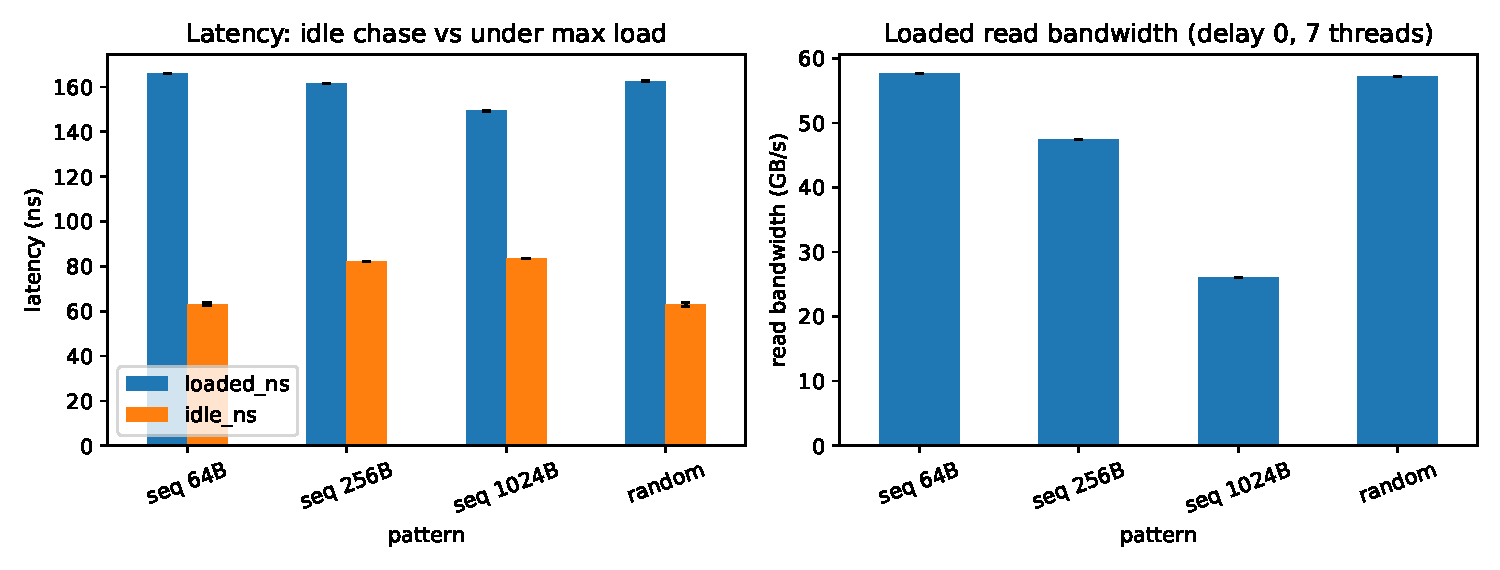
\includegraphics[width=\linewidth]{../plots/pattern_gran.pdf}%
    }
    \caption{DRAM Latency and Bandwidth under Loaded and Idle Conditions. size = 1 GiB}
    \label{fig:pattern-gran}
\end{figure}

When idle, DRAM will perform similar to its zero-queue latency measured
earlier. In fact, we get the same latency (82 ns) for the 256-byte stride and
1024-byte stride sequential patterns as we got for the zero-queue baselines.
When accessing memory in a 64B stride, the memory controller is likely
pre-fetching the next cache line in some cases, improving average latency. It
is not clear why random accesses perform better than the baseline zero-queue
latency, but it is possible that the benchmark hits different channels more
often, and so benefits from memory parallelism.

In the loaded case, the system experiences memory contention, so the latency of
each request increases. Lower strides likely hit the same memory bank
repeatedly, and so increase contention and latency, whereas the higher stride
(1024B) might hit different banks, decreasing contention and latency. It is not
clear, however, why the random access pattern does not benefit from channel
parallelism in the same way we suspect it did in the unloaded case.

We also see that bandwidth decreases as stride increases, but increases again
for a random pattern. As with the latency, we can likely attribute this result
to a balance of pre-fetching and memory parallelism effects.

\begin{figure}[H]
    \makebox[\textwidth][c]{%
        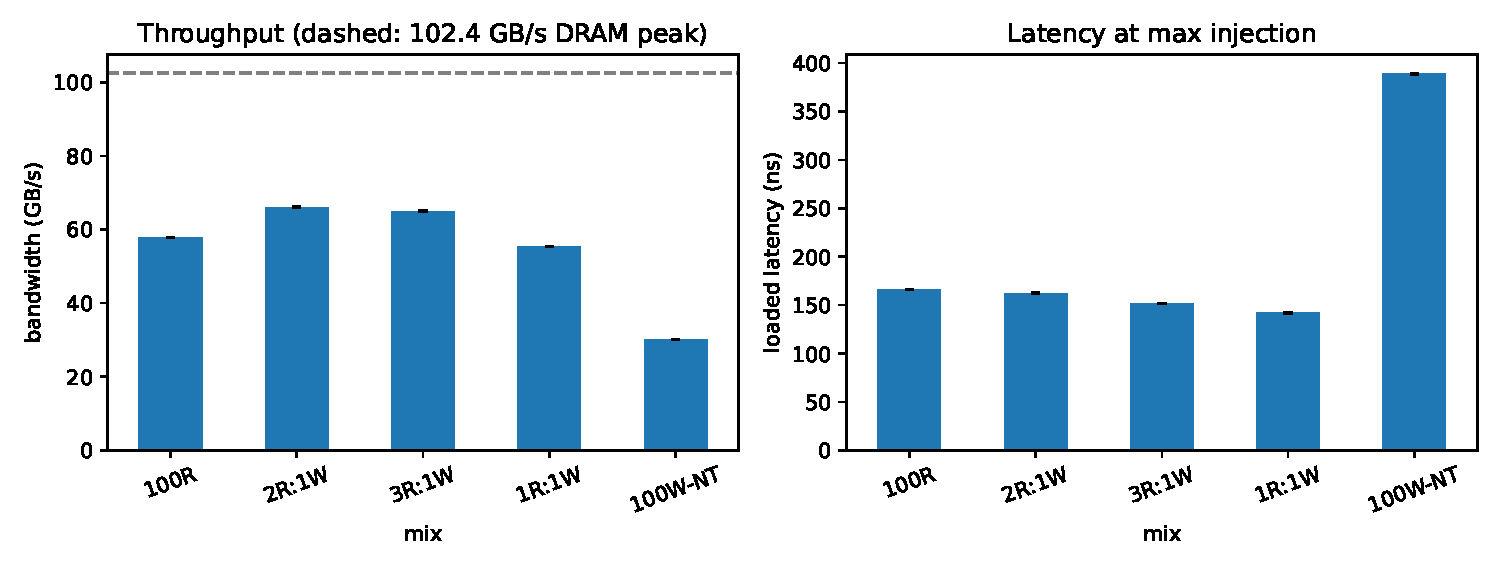
\includegraphics[width=\linewidth]{../plots/rw_mix.pdf}%
    }
    \caption{DRAM Bandwidth and Latency vs. Read/Write Ratio}
    \label{fig:pattern-gran}
\end{figure}

We see that the DRAM performs better in both bandwidth and latency when there
is a mix of reads and writes (with reads preferred over writes). This result is
expected, because reads and writes involve different physical operations in the
DRAM, so the memory controller can more efficiently schedule operations to take
advantage of memory parallelism. The mix also reduces bus contention, because a
write can complete while data is being read back to the CPU over the DDR5 bus.

We also see significantly worse performance for the 100\% writes benchmark.
MLC's 100\% writes are non-temporal. That is, data is always written directly
to DRAM without going through cache. Without the cache, every memory request
must go all the way to DRAM and complete, significantly increasing average
latency and decreasing bandwidth.

\newpage
\section*{Throughput-latency Knee}

\begin{figure}[H]
    \makebox[\textwidth][c]{%
        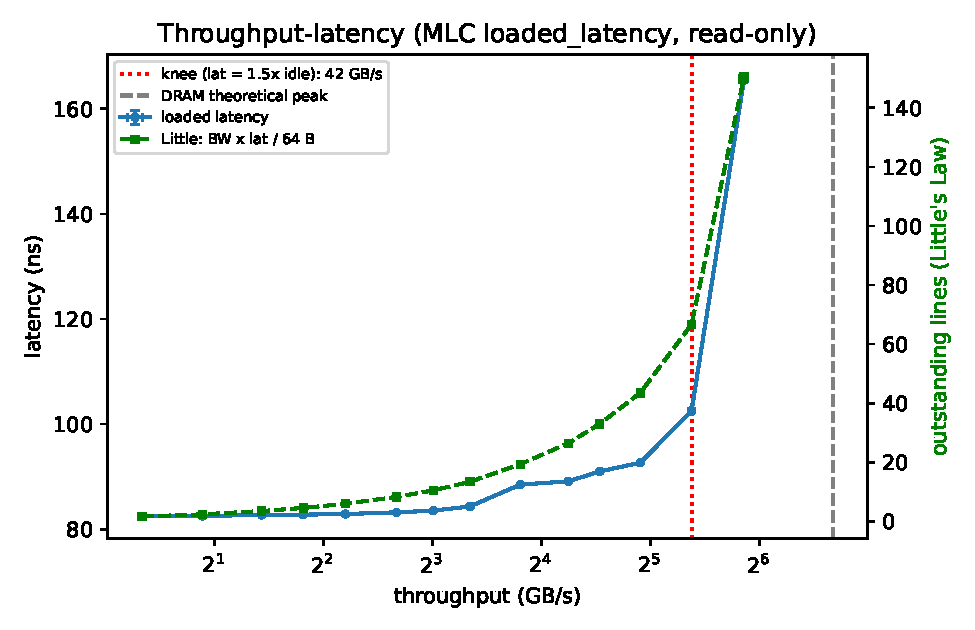
\includegraphics[width=\linewidth]{../plots/intensity.pdf}%
    }
    \caption{Latency and Pending Requests vs. Throughput}
    \label{fig:intensity}
\end{figure}

This experiment sweeps injection delay to achieve a range of throughputs and
latencies. For each throughput-latency combination, we can calculate the number
of outstanding requests ($L$) in the queue using Little's law, as $L = \lambda
W$ where $\lambda=$throughput and $W=$latency.

We see that the number of requests in the queue grows linearly with throughput
until the knee, at which point the queue fills up and the memory controller
forces requests to stall, further increasing the number of in-flight requests.

Latency remains mostly constant (82 ns, same as the zero-queue baseline) while
the number of in-flight requests is below 16 (throughput $\approx$ 12 GB/s).
The access pattern is randomized, so requests likely map to different channels,
banks, and rows, and the memory controller can exploit parallelism to keep
latency down. Past this point, latency begins to rise as memory contention
increases, until the queue fills at the knee, and latency almost doubles
relative to its baseline.


\newpage
\section*{Working-set/Cache/TLB Analysis}

\begin{figure}[H]
    \makebox[\textwidth][c]{%
        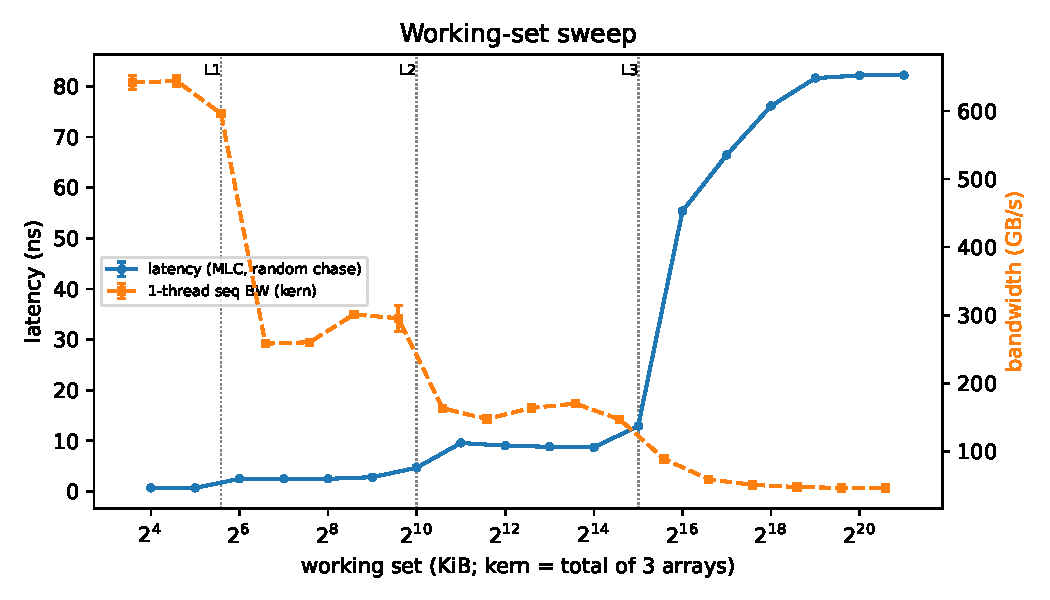
\includegraphics[width=\linewidth]{../plots/working_set.pdf}%
    }
    \caption{}
    \label{fig:working-set}
\end{figure}

The latency figures match the zero-queue baselines exactly, and jump to the
next value when crossing level boundaries. The one difference is that for DRAM,
latency begins at 56 ns for the set twice the size of L3, and then rises with
working set until it flattens out at the 82 ns value observed earlier at around
512 MiB. This effect is likely due to caching. The entire working set cannot
fit in cache, but enough of it does for smaller sizes ($2^{16}$--$2^{18}$ KiB)
that some reads will be orders of magnitude faster and bring down the average
latency.

The bandwidth figures are similar, in that bandwidth is inversely proportional
to latency, but we also get the result that bandwidth increases with working
set within the same memory level. This result is likely caused by pre-fetching
effects, as the memory controller is able to identify the access patterns and
optimize for future elements in the working set.

\begin{figure}[H]
    \makebox[\textwidth][c]{%
        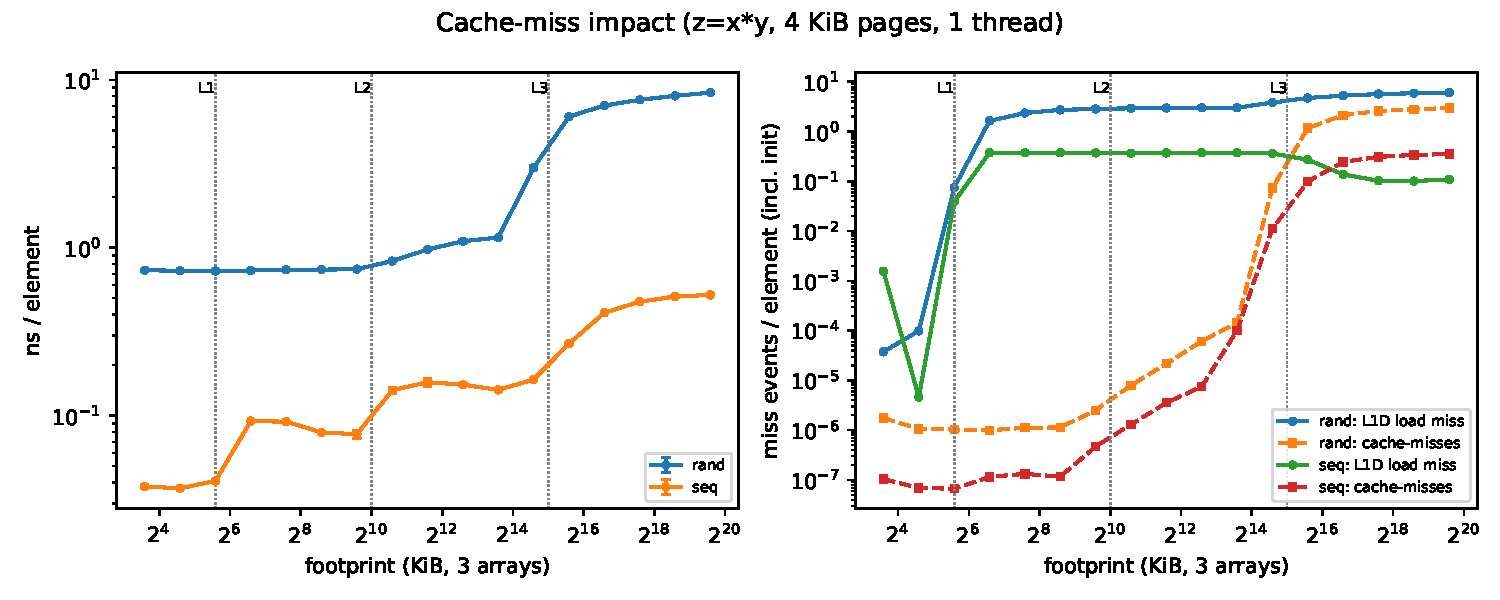
\includegraphics[width=\linewidth]{../plots/cache_miss.pdf}%
    }
    \caption{}
    \label{fig:cache-miss}
\end{figure}

For a random access pattern, we see that each element takes the same latency as
a memory access (same trend as in Fig. \ref{fig:working-set}). This result is
expected, as every element requires 1 memory access, so the kernel is
memory-bound. For the sequential access pattern, the kernel is vectorized and
each memory access is able to load significantly many more elements to be
processed simultaneously. For a more thorough analysis of this behavior, see
the Project 1 Report.

The number of cache misses per element stays mostly constant as the set is L1-
and L2-resident (except for some mandatory misses in the very small 16 KiB
set). In L3, the number of misses slowly increases until it jumps up most
dramatically when the working set no longer fully fits in cache. We see a
similar result for the L1 misses, but the jump expectedly occurs at the L1
boundary. Interestingly, the L1 misses stay constant throughout L2- and
L3-resident sizes, but then increases for random accesses and decreases for
sequential accesses in DRAM. This effect is likely due to pre-fetching. The
DRAM controller is better able to predict pages to cache in the sequential
case, decreasing L1 misses, but the same predictions hurt random access
performance, because the CPU is less likely to need data in nearby pages
shortly.

\begin{figure}[H]
    \makebox[\textwidth][c]{%
        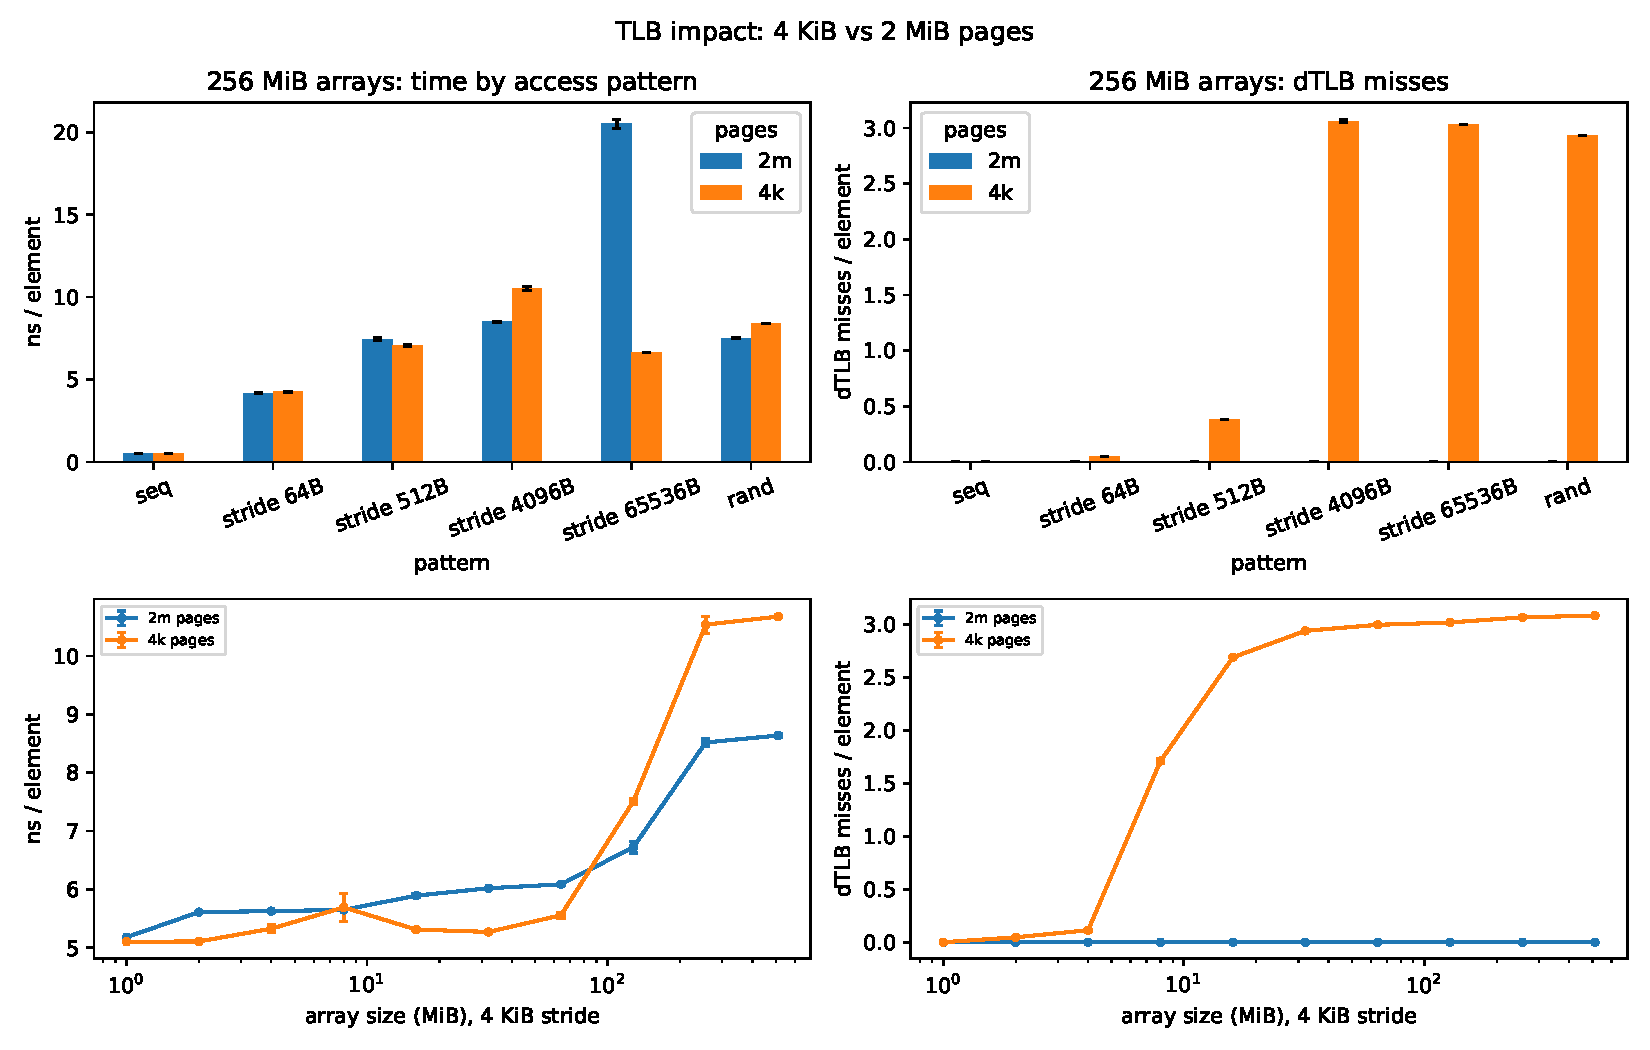
\includegraphics[width=\linewidth]{../plots/tlb.pdf}%
    }
    \caption{Note that the dTLB misses are virtually non-existent for 2 MiB
    pages. The bars can be seen by zooming in sufficiently on the plot.}
    \label{fig:tlb-miss}
\end{figure}

For strides below 4 KiB, the 4 KiB and 2 MiB pages perform very similarly,
albeit with slightly more TLB misses in the 4 KiB case due to crossing page
boundaries. For strides of 4 KiB and above, each element incurs a mandatory 3
TLB misses---one for each array (\texttt{z[i] = x[i] * y[i]}). These misses
likely cause the slight increase in time per element seen for the 4 KiB stride
with 4 KiB pages.

In the 64 KiB case, we see the huge pages perform significantly worse than
regular pages. This result likely stems from how the cache is indexed. The
regular pages map to frames spread throughout the physical address space. Since
the cache is indexed by bits 12 and up of the physical address, the randomness
in these bits results in different indices for each 4 KiB page, so the cache
can store more of the working set even without set-associativity. The 2 MiB
pages, however, map to contiguous frames in the physical address space, and so
bits 12 through 16 stay the same for each element 64 KiB apart. Without full
set-associativity, there is significant contention for the same cache lines,
and so data will be evicted with most accesses.

Huge pages perform best with large working sets and access patterns tuned to
the cache.

\newpage
\section*{Pitfall Analysis}
\begin{figure}[H]
    \makebox[\textwidth][c]{%
        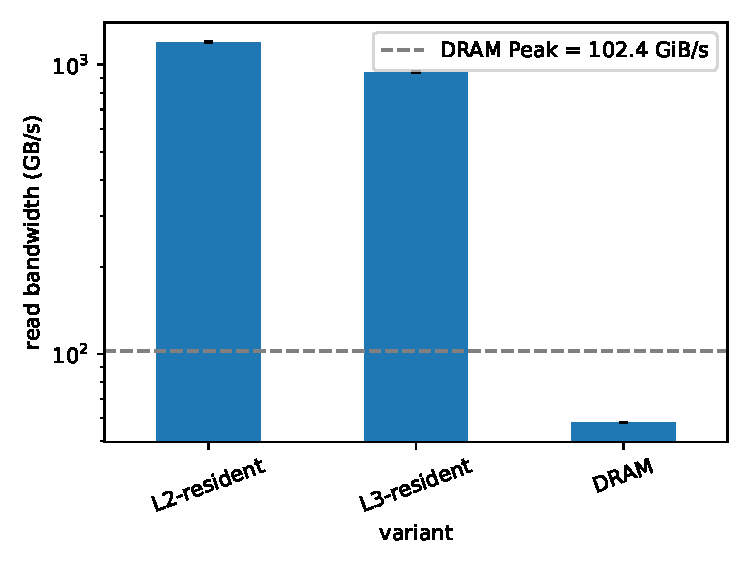
\includegraphics[width=\linewidth]{../plots/pitfall.pdf}%
    }
    \caption{Memory Bandwidth Dependency on Working Set Size.}
    \label{fig:pitfall}
\end{figure}

For each benchmark, it is important to tune the working set size to measure the
intended value. Each memory level operates differently and has different
achievable bandwidths. Measuring "read bandwidth" can mean multiple different
things, and it is not enough to run MLC's bandwidth tool with the default
settings to measure DRAM bandwidth, for example.

\newpage
\section*{AI-use Transparency}

Claude Sonnet 5.5 was used to write all of the benchmark code (shell scripts +
C kernel), as well as most of the Python plotting code. All words in this
report are entirely my own.


% ---- References ----
% \newpage
% \bibliographystyle{IEEEtran}
% \bibliography{references}

\end{document}
